
%(BEGIN_QUESTION)
% Copyright 2014, Tony R. Kuphaldt, released under the Creative Commons Attribution License (v 1.0)
% This means you may do almost anything with this work of mine, so long as you give me proper credit

One of the resistors in this voltage divider circuit is failed open.  Based on the voltage readings shown at each load, determine which one it is:

$$\includegraphics[width=15.5cm]{i01134x01.eps}$$

\underbar{file i01134}
%(END_QUESTION)





%(BEGIN_ANSWER)

Resistor R1 has failed open.  This is evident because only load \#1 is receiving any power; the other two loads are completely ``dead''.

%(END_ANSWER)





%(BEGIN_NOTES)

Discuss with your students how they were able to predict R1 was the faulty resistor.  Is there any particular clue in the diagram indicating R1 as the obvious problem?

%INDEX% Electronics review: series-parallel circuits

%(END_NOTES)


